\documentclass[11pt, a4paper]{article}
\usepackage[left=40mm, right=20mm, top=20mm, bottom=20mm, includefoot]{geometry}
\usepackage{setspace}
\usepackage{graphicx}
\usepackage[english]{babel}
\usepackage[autostyle]{csquotes}
\usepackage{listings}
\usepackage[style=apa,backend=biber, language=english]{biblatex}
\PassOptionsToPackage{hyphens}{url}\usepackage{hyperref}

\addbibresource{sources.bib}
\setlength{\parindent}{0ex}
\setlength{\parskip}{1.5ex}
\font\titlefont=cmr10 at 18pt
\MakeOuterQuote{"}

\lstset{
  frame=tb, % draw a frame at the top and bottom of the code block
  tabsize=4, % tab space width
  showstringspaces=false, % don't mark spaces in strings
  numbers=left, % display line numbers on the left
  commentstyle=\color{green}, % comment color
  keywordstyle=\color{blue}, % keyword color
  stringstyle=\color{red} % string color
}

\linespread{1.5}
\begin{document}

\title{\titlefont The path to the right decision: An investigation into using heuristic pathfinding algorithms for decision making in game AI}
\author{Ashley Smith}
\date{\today}
\maketitle
\thispagestyle{empty}

\renewcommand\abstractname{\textbf{Abstract}}
\begin{abstract}
Lorem ipsum dolor sit amet, consectetur adipiscing elit. Cras justo velit, vestibulum sit amet turpis in, interdum rhoncus magna. Proin pulvinar posuere iaculis. Duis vulputate tristique arcu, id pretium ante blandit ut. Vestibulum ante ipsum primis in faucibus orci luctus et ultrices posuere cubilia Curae; Nam augue tellus, mattis quis consequat id, facilisis eu lectus. Vivamus euismod non quam sed condimentum. Orci varius natoque penatibus et magnis dis parturient montes, nascetur ridiculus mus. Orci varius natoque penatibus et magnis dis parturient montes, nascetur ridiculus mus. Phasellus vitae consequat nisi. Morbi vulputate tellus ut nibh vulputate, vitae blandit ex faucibus.
\end{abstract}

\cleardoublepage
\setcounter{page}{1}
\pagenumbering{roman}
\tableofcontents

\cleardoublepage
\pagenumbering{arabic}
\setcounter{page}{1}

\section{Introduction}
\label{sec:introduction}

\subsubsection{Video games and artificial intelligence}
\label{subsubsec:videoGamesAndAI}

Games are good for the global economy. \citeauthor{Newzoo} \parencite*{Newzoo} reports that in October 2019 the global games market was worth \$148 billion. In order to remain competitive, developers are pushed to make bigger, better and more complex games. The evolution of the technologies available has allowed for a greater number of elements to be simulated in the game world which could potentially increase a game's worth \parencite{blow2004game}. The entry barrier to creating these good-looking and well executed games has been lifted with the establishment of engines like Unity \parencite{Unity} and Unreal \parencite{Unreal} to the point where even non-programmers can get involved using textual or visual scripting.

For many years, only the game's graphics were considered important \parencites{yap2002grid, blow2004game}, however, good physics systems or competent AI (Artificial Intelligence) are now recognised as a way of improving the end-user's experience just as much \parencite{blow2004game}. Game AI is different from the normal, academic AI as it simulates behaviour and aims to be believable and fun, whereas an academic AI aims to achieve a level of intelligence or autonomy to excel at a given task \parencite[60]{nareyek2004ai}.

\subsubsection{The need for game AI}
\label{subsubsec:theNeedForGameAI}

AI has multiple uses within a games context but the majority of use cases employ AI to control the characters featured in a level of the game. \citeauthor{laird2001human} \parencite*[16]{laird2001human} said that whether these characters are replacements for opposing players or characters that act as companions, villains and plot devices, "human-level AI can expand the types of experiences people have playing computer games". Using AI opens up the opportunity for increasing the difficulty of the game, and could be perceived as the kind of challenges that make games fun \parencite[2]{buro2004call}. \citeauthor{laird2001human} \parencite*[16]{laird2001human} also hypothesised that utilising such an AI is a good step towards the development of enjoyable and challenging gameplay, and potentially to "completely new genres" \parencite[17]{laird2001human}.

 "Customers value great AI" \parencite[60]{nareyek2004ai} and so it's important to choose a suitable approach that fulfils the expectations of the player thus the requirements of the game \parencite[19]{millington2019ai}. Academic AI can be made using algorithms inspired by biology such as neural networks or genetic algorithms and trained through iteration or with datasets. These approaches aren't used in game AI because of the high requirements to train the AI to interact with a specific game \parencite[64]{nareyek2004ai}, moreover, it is easy to train the AI to play too strongly ruin the game \parencite[13]{tozour2002evolution}. Instead, game AI developers embrace simpler, non-learning algorithms due to them being easier to understand, implement and debug \parencite[7]{tozour2002evolution}.

\subsubsection{Approaches to game AI development}
\label{subsubsec:approachesToGameAIDevelopment}

The most basic forms of AI used in games take the form of a series of if-then statements and are known as `production rule systems' \parencite{tozour2002evolution}. These statements are organised in a list and the AI uses the behaviour of the rules that evaluate to $true$. The result is a very basic AI that is not only limited to what actions it can take but also when it can take them. Similarly, decision trees combine the same if-then style with branching structures to create game AI \parencite[62]{nareyek2004ai}, and the tree and subtrees are recursively traversed until a leaf node is found with the desired behaviour. This process is very easy to understand and implement \parencite[295]{millington2019ai}, and the branching structure makes visualisation of the process more intuitive than the basic list used in a production rule system. Because of this, many consider decision trees to be one of, if not the simplest techniques to making AI  (\cite[295]{millington2019ai}; \cite[7]{tozour2002evolution}).

\emph{TODO: DIAGRAM OF DECISION TREES HERE}

FSMs, or Finite State Machines, are the most common approach to game AI (\cite[1]{orkin2006three}; \cite[309]{millington2019ai}) due to being easy to understand and the efficacy of their output. FSMs consist of a directed graph where each node represents a state and the edges represent the transitions between them \parencite[6]{tozour2002evolution}. A character can only be in one state at time and has no memory of any previous states \parencite{colledanchise2014performance}; each state represents an expected behaviour and determines what they do and the conditions to switch to a different state \parencite[3]{diller2004behavior}. In the right environment, the impression of a well thought out FSM could compete with that a neural network, at a fraction of the time and resource costs, despite not always arriving at the optimal decisions \parencite{sweetser2002current}. However, each new behaviour requires the creation of a new state and the conditions of which this state integrates and transitions into other states, making expansion and maintenance cumbersome (\cite[2]{sweetser2002current}; \cite[3]{lim2010evolving}). There's no easy way to combine the tests inside of FSMs and selecting the conditions for a state transition is still very much a process that must be done by hand \parencite[313]{millington2019ai}. 

\emph{TODO: FSM DIAGRAM}

The need for more flexibility in game AI has lead to the creation adaptation of modular algorithms such as behaviour trees \parencite[1]{lim2010evolving}. Like decision trees, the recursive structure of a behaviour tree is simple to understand and implement while also being high level, allowing for more sophisticated AI to be created in a modular fashion through the use of subtrees and different node types \parencite[144]{shoulson2011parameterizing}, each performs an action or check and then proceeds to succeed or fail \parencite[4]{lim2010evolving}. It is these types that make the AI process at a higher level than standard decision trees, and when combined with leaf nodes that perform checks and actions to build trees, and then combined again to make trees containing subtrees, the simplicity and elegance of this technique certainly demonstrates why behaviour trees are getting attention \parencite[144]{shoulson2011parameterizing}.

\emph{TODO: BEHAVIOUR TREE DIAGRAM}

\subsubsection{The relationship of pathfinding and game AI}
\label{subsubsec:theRelationshipOfPathfindingAndGameAI}

One common requirement for game AI is for the characters to be able to traverse the areas of the game in a way which meets the player's expectations logically and efficiently --- a task known as pathfinding. Regardless of what an AI decides to do, a pathfinding mechanic needs to be in place to allow the AI to navigate to where it needs to go, manoeuvring around obstacles while still taking a sensible route \parencite[60]{graham2003pathfinding}. For most games, the algorithm of choice is A* as it is the de-facto standard pathfinding algorithm (\cite[197]{millington2019ai}; \cite[2]{botea2004near}; \cite[64]{nareyek2004ai}; \cite[73]{leigh2007using}).

The A* algorithm analyses the game's map and generates a path from one location to another while minimising a $cost$ value --- this value can represent anything but usually it represents the time or distance to travel along a given route \parencite[44]{yap2002grid}. This means that the pathfinding algorithm itself doesn't decide where to go, only how to get there and the manner in which it does so. When asked to calculate a path, a pathfinding algorithm is provided a graph of nodes to determine which nodes can be reached from which \parencite[61]{nareyek2004ai}. The algorithm isn't concerned in what the data represents (2D or 3D coordinate data), the data's form (a tree, a graph or a list of connections) or the unit of measurement to calculate the weight of an edge (length, traversal time or monetary cost), as long as it is equipped with the right functionality to digest this information (\cite[277]{millington2019ai}; \cite[60]{graham2003pathfinding}).

With the pathfinding process taking place after the decision has been made, the opportunity to involve the data gathered from pathfinding algorithm is missed. Often, the AI will decide to approach the nearest object, but obstacles in the way mean that the cost of navigating to the destination is greater than some alternative. While implementing the algorithm isn't difficult, ensuring the AI generates a path to the correct destination is difficult to do well \parencite{forbus2002qualitative}. Perhaps on the way to the destination, the character has to also navigate past traps or other hazards where it will need to decide whether to avoid or pass through --- decisions that A* isn't fully equipped to deal with on it's own. If the AI wanted to factor in these hazards and real cost values, it would have to perform a more advanced check on where to travel too, maybe even using the pathfinding algorithm multiple times to definitely make sure that it wants to take the generated path, potentially ruining the game's speed and overall performance.

Pathfinding algorithms are actually general purpose search algorithms applied to a spatial context (\cite[125]{cui2011based}; \cite[6]{orkin2003applying}; \cite[46]{yap2002grid}); there is no such restriction that these algorithms should be limited to pathfinding when in a games context. \citeauthor{millington2019ai} \parencite*[197]{millington2019ai} said that "pathfinding can also be placed in the driving seat, making decisions about where to move as well as how to get there". With search algorithms having the flexibility of being able to traverse graphs of nodes representing any kind of data, it's no stretch to imagine the A* search algorithm being applied to a graph containing the same tests and actions found in decision and behaviour trees in order to generate a `path' of actions rather than a path of spatial data \parencite[114]{higgins2002generic}. This is paper aims to investigate and re-engineer A* to make decisions rather than paths in a game context.

\subsection{Literature Review}
\label{subsec:literatureReview}

\subsubsection{Dijkstra's algorithm: A graph and tree search algorithm}
\label{subsubsec:dijkstrasAlgorithm}

A search algorithm is a recursive method designed to find a match for a piece of data within a collection such as an array, graph or tree \parencite{friedman1976algorithm}. A piece of data is provided and the search algorithm typically returns whether it is present and it's location. \citeauthor{dijkstra1959note}'s algorithm \parencite*{dijkstra1959note} is a search algorithm that operates on trees and graphs (which are then interpreted as trees). The algorithm calculates the shortest difference from any node on the graph to any other node, and can be terminated early to avoid unnecessary computation if a destination is provided and found.

Dijkstra's algorithm works through the recursive summation and comparison of distance values starting from the a given start node \parencite[269]{dijkstra1959note}. Each neighbouring node is added to the \emph{open} list, then, the current node's distance from the start is added to the length between the current node and its neighbour. If this tentative value is lower than the current distance value of the neighbour, it replaces it. When all the neighbours have been considered, the node with the lowest tentative value on the graph is selected and permanently `visited' and are removed from the \emph{open} list \parencite{dijkstra1959note}. This process is repeated until either there are no \emph{open} nodes left or the destination, if provided, has been visited, and thus a path and the distance from the start to the destination can be retrieved. The problem with Dijkstra's algorithm is that it always selects the node with the lowest tentative distance value, meaning that the algorithm has no notion of direction and is calculating the lowest distance to nodes that may not be relevant to getting to the destination \parencite[214]{millington2019ai}.

\emph{TODO: DIJKSTRA'S ALGORITHM DIAGRAM}

\subsubsection{A* algorithm: A heuristic best-first search algorithm}
\label{subsubsec:aStarAlgorithm}

A* is an improvement of Dijkstra's algorithm in this regard \parencite[101]{hart1968formal} --- while it doesn't stray far from how Dijkstra's algorithm works in the sense that it operates using a tentative distance value and it keeps track of the nodes that have and haven't been visited, it does extend the algorithm using what's known as a heuristic approach \parencite[126]{cui2011based}. "Heuristics are criteria, methods or principles for deciding which among several alternative courses of action promises to be the most effective in order to achieve some goal" \parencite[3]{pearl1984heuristics}. This means that in a pathfinding situation, a heuristic function could estimate the distance to the goal, by ignoring walls and measuring in a straight line, to direct the algorithm in the right direction and avoid evaluating routes that travel in the wrong direction to make the process more efficient \parencite[127]{cui2011based}. Heuristics enable A* to perform a best-first search \parencite[46]{yap2002grid}, as the heuristic now has the power to select which node is the best to evaluate and prioritise over the others \parencite[94]{russell2016artificial}.

When identifying the next node to expand, A* will take this heuristic distance into account using the formula $f(n) = g(n) + h(n)$ (\cite[102]{hart1968formal}; \cite[95]{russell2016artificial}), where $g(n)$ is the real distance the algorithm has calculated from the start node to node $n$ and is the distance to be minimised while finding the \emph{goal}, $h(n)$ is the \emph{heuristic} distance from the current node $n$ and the destination, and $f(n)$ is the combination of these two metrics forming an estimate of the distance from the start node to the destination if travelling through node $n$, also known as the \emph{fitness} value (\cite{hart1968formal}; \cite{millington2019ai}; \cite[64]{graham2003pathfinding}). 

This heuristic component of A* transforms it into a family of algorithms where applying a different heuristic selects a different algorithm \parencite[107]{hart1968formal}, moreover, implementing A* and using a heuristic that returns a constant value for all nodes reverts A* back into Dijkstra's algorithm (\cite[10]{lester2005pathfinding}; \cite[237]{millington2019ai}). Conversely, implementing a well-designed heuristic method can be used to guarantee optimal solutions, and using a heuristic that is somewhere in-between can output results with varying degrees of accuracy in exchange for faster execution \parencite[219]{millington2019ai}.  The implementation of a good heuristic can be difficult, as making the heuristic take more factors into account for accuracy has the drawback of making the algorithm less efficient overall with the heuristic being frequently used throughout the process.

On the other hand, \citeauthor{graham2003pathfinding} \parencite*[68]{graham2003pathfinding} argue that one of the constraints of games the industry is the "over-reliance" on the A* pathfinding algorithm and describe the development of its many extensions as a way of avoiding the discovery of new techniques. The pathfinding process can require a lot of CPU resources, sometimes to the point of stalling the game, when applied to larger graphs (\cite[127]{cui2011based}; \cite[110]{stentz1996map}; \cite[67]{graham2003pathfinding}). This indicates that the performance of A* can vary depending on various factors, and is why it is important to optimise A* by selecting an suitable storage mechanism for the graph and internal node storage as well as using a reasonable heuristic that balances efficiency and efficacy \parencite[228]{millington2019ai}.

\emph{TODO: CRITICAL: A* DIAGRAM}

\subsubsection{Processing a character's perception of the game world}
\label{subsubsec:processingACharactersPerception}

These approaches need a way to digest information about the character and its environment that is relevant to the decision making process, and selecting this information is just as important as the form it is delivered in \parencite[126]{cui2011based}. This extraction of world data can vary in difficulty \parencite[3]{diller2004behavior} and is done for both performance and gameplay needs. All game AI solutions need the world to be re-interpreted to be better suited for both decision making \parencite[2]{buro2004call} and pathfinding \parencite[3]{diller2004behavior}. Particular geometry of the map may need to be interpreted as vantage points, choke points or safe spots; particular formations of enemy units may need to be not only counted but also assessed for tactical strengths, whether engaging the units head-on is better than running away to a better location, and finally, the interpretation of time such as whether there is enough time to navigate to what would otherwise be a better location for fighting the enemy \parencite{buro2004call}. An AI would then take this abstraction of the world, combine it with the character's data and then consider what the character should be doing --- if the character is in an `attacking' state and the player is nearby then the decision would involve getting into a position and hitting or shooting at the player. 

If A* is to be used for game AI it also needs to operate on non-positional data. In standard pathfinding, each node is a position in the world and the edges between these nodes are the movements to get from one to another. Substituting each node to be an AI state and each edge to be an action that causes transitions from one state to another creates a graph that A* could process. The implementation the states and actions depend on the expectations of the AI --- traditional pathfinding could be implemented by having an action that triggers movement and changes the position variable in the character's state. Regardless, a graph consisting of these nodes could be difficult to process and reduce the speed of A*.

A* can suffer from performance problems when used with many agents at once, or with a large or inefficient graph of nodes \parencite{graham2003pathfinding}. Many solutions have been discovered to prevent or reduce the impact on performance --- one such solution is known as hierarchical pathfinding, where the game's map is simplified into chunks, \parencite[126]{cui2011based}. By simplifying a group or grid of nodes into a single node that represents the whole group (like a quadtree), the pathfinding process can be applied to larger worlds as if they were actually smaller \parencite{botea2004near}. This works well for standard pathfinding, but if A* is applied to something other than purely spatial world data then the nodes need extra consideration. 

\emph{TODO: DIAGRAM ABOUT HIERARCHICAL PATHFINDING}

There is a large amount of actions a character can take at any given moment \parencite[62]{nareyek2004ai} and so applying a search algorithm to such a large set of tasks will make the process a lot slower than traditional methods if left unchecked. Hierarchical pathfinding essentially creates more nodes to expand in the short term to reduce the total number of nodes expanded in the long term and gain a net increase in performance. If hierarchical pathfinding reduces the amount of destinations, by collecting connections between the nodes in a given area, and simplifies navigation to and from this area then this technique can also be applied to the character's state so long as these connections can be aggregated using other metrics other than purely relying on their proximities to each other. One such way of grouping  could be separating `attacking' actions from `defending' actions so that character's deciding to play defensively can eliminate one route of evaluation rather than multiple. Splitting gameplay elements like this can get complicated --- if a certain unit in a strategy game can attack from a longer range, would attacking the enemy from a distance be a defensive manoeuvre or an offensive one, and how easy is this to change on a per-unit basis \parencite{weber2011building}?

\subsubsection{Making decisions with A* using GOAP}
\label{subsubsec:makingDecisionsWithAStarUsingGOAP}

\citeauthor{orkin2003applying} \parencite*[11]{orkin2003applying} expressed that expectations of AI are growing with the release of every new game and that "we need to look toward more structured, formalized solutions to creating scalable, maintainable and re-usable decision making systems". Techniques used to create the Game AI featured in most games do not contain the scalability \citeauthor{orkin2003applying} envisions \parencite[17]{laird2001human}, however, \citeauthor{higgins2002generic} \parencite*[117]{higgins2002generic} declares that a pathfinding engine can be created generically, especially if a templated language is used, to give the code even more reusability. Implementing A* in this way would allow it to be used for both regular pathfinding and anything else that could requires searching \parencite[120]{higgins2002generic}. With A* being efficient and optimisable \parencite[215]{millington2019ai}, reusing A* for game AI has the potential to bring the benefits it usually brings to pathfinding to AI while being adaptable enough to scale up and meet expectations.

\citeauthor{orkin2006three} \parencite*[1]{orkin2006three} worked on the development of the game AI for the game F.E.A.R \parencite{FEAR}. The approach used for this AI was called GOAP which stands for `Goal Oriented Action Planning' and uses the A* algorithm as part of its decision making process and "allows characters to decide not only what to do, but how to do it" \parencite[1]{orkin2003applying}. GOAP changes the data to be processed by A* from spatial data such as coordinates into character AI state data, such as what is found in FSMs. Therefore, the output of A* is no longer a sequence of movements but a sequence of actions also known as a plan (\cite[2]{orkin2003applying}; \cite[6]{tozour2002evolution}).

GOAP essentially takes the idea of having state machines to encapsulate behaviours and replaces the hand-programming the conditions and connections of state transitions with a pathfinding process with the aim being the decoupling of states and their transitions \parencite[2]{orkin2003applying}. The pathfinding process uses each node to represent a state and the edges between each node as the actions that lead to those states \parencite[7]{orkin2003applying} When GOAP is used, a goal is given for the character to achieve, which drives the AI to play the game rather than idly remain inactive, and what is returned is the sequence of actions that will satisfy the goal \parencite[1]{orkin2003applying}. An action is a representation of one thing the character will do to change the world in some way, like opening a door or picking up a weapon \parencite{orkin2003applying}; some actions have preconditions that require the execution of another action prior to it \parencite[5]{orkin2003applying}. A* will then find the sequence of actions, the plan, that satisfies the character's goal while minimising an arbitrary $cost$ value --- \citeauthor{orkin2003applying} \parencite*[4-5]{orkin2003applying} suggests that this process creates interesting character AI that can adapt to change while also having a code structure that is reusable, maintainable and "elegant".

\begin{figure}[h]
  \centering
  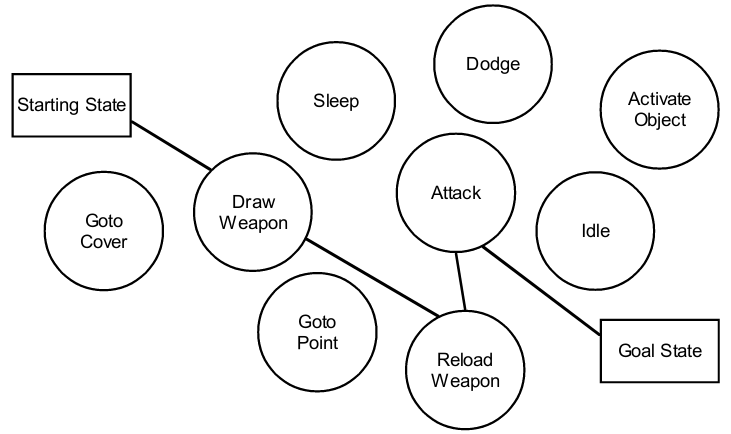
\includegraphics[width=\linewidth]{img/goap.png}
  \caption{An example of GOAP \parencite[3]{orkin2003applying}}
  \label{fig:goap}
\end{figure}

A* being used in GOAP means that fundamental formula $f(n) = g(n) + h(n)$ \parencite[102]{hart1968formal} is implemented in a way such that A* can perform a best-first search and expand the actions that are more likely to be  useful to the situation \parencite[7]{orkin2003applying}. To calculate $h(n)$, \citeauthor{orkin2003applying} \parencite*[7]{orkin2003applying} also shares that the heuristic in GOAP can be calculated as the summation of unmet conditions of the goal node, but this is rather unclear. Given the example in figure \ref{fig:goap}, "the goal is to kill an enemy" \parencite[3]{orkin2003applying} could be interpreted in various ways that all seem unsuitable. If the goal condition is that the enemy is dead, the heuristic would be the same for all nodes but the goal state, making it potentially wasteful like Dijkstra's algorithm \parencite[214]{millington2019ai}. Alternatively, if the condition was divided into multiple conditions such as the weapon needing to be drawn, the weapon needing to be loaded, and the enemy being dead, it is implied that either the algorithm has been run previously to determine the requirements of killing an enemy, or that they were programmed by the programmer --- how would the starting state know that the weapon needed to be reloaded before drawing it? While GOAP does seem elegant, the graph in figure \ref{fig:goap} doesn't have a sizeable number of nodes; using Dijkstra's algorithm wouldn't incur much of a performance cost with a graph this size. \citeauthor{orkin2003applying} \parencite*{orkin2003applying} suggests that a regressive search by starting at the goal and pathing to the start makes sense, and in figure \ref{fig:goap}, it does, as only one action can attack and so it's clear that the decision making process boils down to the character attacking the enemy.

Another problem of GOAP is that the high-level nature of the approach may not allow for enough control of the game \parencite[87]{stanciu2012implementing} --- while making abstractions of the world is necessary for AI to process the information \parencite[2]{buro2004call} and thinking on a higher level is beneficial for making more human-like decisions, the precision of the actions taken by the AI is both low level and very noticeable if incorrect \parencite[60]{graham2003pathfinding}. Figure \ref{fig:goap} shows a decision making process that decides what to do but not necessarily where to do it. When the action "Goto Point" in figure \ref{fig:goap} gets executed, there's no indication of how the destinations are generated other than satisfying the preconditions for another action (for example, moving to an object to activate it) \parencite[7]{orkin2003applying}. 

This isn't specific to GOAP as it applies to every AI approach where the generation of these locations isn't part of the AI. Is the character's AI deciding where to go, or just deciding that it has to go somewhere? In order for "Goto Cover" to act in a similar way to the "Goto Point" action, a goal or action precondition would either have to require the character to be out of line-of-sight, or be using one of the designated cover spots --- this is how F.E.A.R \parencite*{FEAR} approached it \parencite[12]{orkin2006three}. The former would require calculating the closest position that allows the escape of line-of-sight. The latter of these would require set locations to be marked as points of interest and then A* would be employed to find which cover spot would be the quickest to navigate to. Both of these would have their own problems, and wrapping the entire pathfinding process as a single action would mean that the information from the pathfinding request would not be used in the decision making at all. Without utilising the AI's ability to create an impression of thought, the information given to these actions could be poorly chosen and "may be perceived as a lack of intelligence by a human player" \parencite[63]{graham2003pathfinding}.

\subsubsection{Defining the notion of cost in the context of game AI}
\label{subsubsec:definingTheNotionOfCost}

$Cost$, sometimes referred to as weight, is a term that will continue to be used when talking about A* as it is the the metric that governs the searching process \parencite[60]{graham2003pathfinding}. $Cost$ doesn't have to be a numeric value, as long as it can be compared and combined correctly with other $cost$ values, however, one numeric restriction of cost is that it cannot, or rather should not, be negative. The method A* uses to determine if a route should be expanded before another is if its $cost$ value is lower --- when only positive values are added together it is assumed that there isn't a way for a $cost$ to decrease in value. While in mathematics it is entirely possible and valid for these values to be negative, the problems that make this necessary are not applicable to games \parencite[202]{millington2019ai}.

In the formula $f(n) = g(n) + h(n)$ \parencite{hart1968formal}, each function returns a $cost$ --- the combination of the goal and heuristic $cost$ values, also known as the fitness value, is used select the next open node to evaluate \parencite[94]{russell2016artificial}. If $a$ and $b$ are two nodes in a graph and $f(a) < f(b)$, A* will interpret this as node $a$ being a more logical choice to expand \parencite[7]{orkin2003applying}. Node $b$ won't be evaluated unless the route derived from node $a$ results in dead ends or more routes which have worse fitness values than node $b$. With the order of execution being so dependent on $f(n)$, it is important that the definition of the $cost$ of an action is calculated correctly. It is difficult to design such a system when everything is arbitrary, but metrics such as distance can be used to prioritise actions with lower distances such as movement; resources such as gold or mana could be used in game specific interactions to minimise spending important resource, and the time spent doing the action can also be factored in to drive the character to resolve the situation as quickly as possible \parencite[8]{lester2005pathfinding}. \citeauthor{millington2019ai} \parencite*{millington2019ai} said that "the cost function is a blend of many different concerns, and there can be different cost functions for different characters in a game" and that this is called "tactical pathfinding". The ability to change the $cost$ per character further demonstrates the adaptability of A* --- changing the way a character interacts with the world is just changing these $cost$ functions so that the A* prioritises one action over another.

Some decisions are more troublesome to weigh than others. With the constraint of no-negativity, what would the $cost$ be of an ability that regenerates mana instead of expending it? The only way apply reductions to values in this way would be to have a baseline $cost$ for an action and then add or subtract from it, however, this does mean that this baseline value would dictate the maximum value of the reduction and so forward planning is necessary to ensure that all reductions can be applied in a balanced way. Another difficult type of decision to way are ones that don't have inherent characteristics; with a good goal for AI being unpredictable, surprising behaviour \parencite[17]{scott2002illusion}, how would the incentive for performing strategies like flanking and ambushing be created, and how would it compare to the $cost$ for attacking an enemy directly head-on? \citeauthor{orkin2006three} \parencite*[14]{orkin2006three} said that in F.E.A.R \parencite{FEAR} this behaviour just came naturally from using a dynamic decision making system such as GOAP and that while they were prepared to implement "complex squad behaviour", none was implemented --- the squad's ability to ambush "emerged" from the combination of the "squad level" decisions and the individual character's decisions which gave the illusion of complex behaviour. \citeauthor{orkin2006three} doesn't mention much more on this subject and so GOAP's ability to surprise remains uncertain.

\citeauthor{harmon2002economic} \parencite*[405]{harmon2002economic} suggests that an "opportunity cost" could be introduced which represents the other actions that cannot be taken as a result of taking the given, mutually exclusive action, the objective being to apply penalties to actions due to the fact that an alternative and possibly better course of action is available. While this makes sense when it is difficult to reward the AI for performing these strategies, but adding penalties to other actions could get complex, there is no discussion of this concept from \citeauthor{orkin2006three} \parencite*{orkin2006three} from his work on F.E.A.R. Although, it is unclear whether \citeauthor{harmon2002economic} means to apply penalties based on the current action or the other actions, and if it's the latter, is this a flat $cost$ shared amongst all actions or does it try to give smaller penalties to the better tasks somehow? Regardless, to calculate this $cost$ some mechanism of the AI, such as the weighting function used to determine $g(n)$ or possibly the nodes themselves, needs to have knowledge of other nodes so that this opportunity cost can be determined and used, yet again requiring forward planning.

GOAP uses a simple "action cost" system to prioritise which tasks to carry out first \parencite[11]{orkin2006three}. Using an integer or floating point value is ideal for the type of $cost$ as it can be added and compared with other values trivially. However, GOAP's method of creating unique characters is to assign different actions to make them act differently \parencite[8]{orkin2006three} as opposed to having them evaluate situations differently as \citeauthor{millington2019ai} \parencite*{millington2019ai} suggested. Giving characters different actions will implicitly change how they prioritise the same situation as they will be given new routes to explore, and for most games this might be the best idea. It could be a good idea to split the $cost$ type into a set of values to give actions different values. Throwing a grenade and shooting a pistol could be considered equivalent in difficulty to perform, but typically grenades have more firepower in exchange for there being less available; reducing these actions to a single value could be difficult depending on the approach, but splitting the value into a set would allow the programmers to keep track of firepower and usage penalties separately. When needed for comparison, this set would evaluate to the sum of it's parts --- but certain characters or situations could choose to adjust or completely omit parts of the $cost$ so that actions are perceived in different ways depending on how a character views a certain cost. For a fast character, the $cost$ to move might be halved and the $cost$ of being exposed doubled in order to give the impression of an agile and hard-to-hit character.

\subsubsection{Generation, selection and application of goal state nodes}

When the game world has been processed, the actions a character can perform have been laid out and the methods of evaluating courses of action have been provided, the only things remaining that A* needs to function are the start and goal node states for the actual decision. The starting state is trivial as it is simply the current state of the character and world; the goal state node requires more consideration than that though. In standard pathfinding, the output is the shortest path from the starting node to the goal node, if such a path exists \parencite[61]{nareyek2004ai}. For game AI though, the goal needs to represent how the character or world should be --- or rather the objective outcome of the decision making process. This objective can be difficult to ascertain as a goal node could represent anything; what seems to be a simple goal such `win the game' becomes a rigorous series of tests to both calculate the $cost$ reaching the goal than another \parencite[403]{harmon2002economic}. On the other hand, objectives that are too small or disconnected may not combine correctly to form this over-arching goal of winning the game. A balance is needed, whether that means the objective is to chase the player or defend an area, the objective needs to be focused on winning without being vague.

While \citeauthor{orkin2003applying} \parencite*{orkin2003applying} talks about in great depth about how GOAP handles making a decision to satisfy goal conditions, but doesn't describe where these objectives come from. A "squad coordinator" is mentioned \parencite[13]{orkin2003applying} that organises multiple agents into squads when they're close together, but the actual goals of the AI can come from both the character's individual AI and the squad coordinator. GOAP doesn't replace an FSM, so it could be inferred that the character's state when a goal is reached determines the next goal and thus the character's behaviour, with the initial state being defaulted, scripted or randomised \parencite[2]{orkin2003applying}. Alternatively, game AI could be created in layers, and the output of one layer could be the desired goal of another, but this would mean that this problem propagates to the highest level. 

Another talking point regarding goals is the amount of designated goal state nodes in the graph. There is typically only a single goal in standard pathfinding, but it is possible, maybe even advantageous, for some games to contain multiple goal nodes in a graph \parencite[272]{millington2019ai}. Instead of checking for a match with a certain location (or state, when developing AI), a method that checks whether a given node meets the requirements of being classified as a goal could be used instead; the heuristic would also need revision as it would need to calculate the heuristic $cost$ to reach the 'nearest' goal rather than just the single, given goal \parencite[272]{millington2019ai}. Having multiple goals and goal types \parencite[121]{higgins2002generic} would grant the ability for the AI to re-route to a different goal if it's easier and therefore accomplish the same task in multiple different ways without creating generic goals; this has its drawbacks though, one being the need for a more intricate and potentially confusing implementation and design of the AI needs, the other being the creation of balancing difficulties to ensure goals are prioritised as expected.

\subsubsection{Summary}
\label{subsubsec:litReviewSummary}

Search algorithms such as A* are generic, maintainable and versatile and are therefore theoretically suitable replacements for FSMs and behaviour trees for implementing game AI. While GOAP does use A* for part of it's decision making process, it isn't a complete solution and still separates decision making from the pathfinding process. This is acceptable and valid as GOAP is for generating a sequence of actions whereas pathfinding is strictly for navigating the map in order to perform these actions. Unfortunately, some information found during pathfinding that could be considered useful for decision making is lost unless explicitly communicated --- a decision might request to navigate to some location, but the path generated might be longer than expected and a different course of action could have been more appropriate. Without replanning, GOAP's disconnect between these systems could result in the wrong decisions being made.

In this paper, the mechanisms of the A* search algorithm are examined and re-engineered, through the substitution of input and output types, to investigate the modularity and adaptability of an AI that uses search algorithms to make decisions while actively involving pathfinding in the process as opposed to keeping these systems separate. Several approaches to defining goals and heuristic methods will be used to visualise the effects they have on a squad-controlling game AI. The aim of using this approach is to bring decision-making and pathfinding closer together and therefore simplifying the overarching process of perceiving, deciding and interacting in the game world.

\subsection{Methods and Methodologies}
\label{subsec:methodsAndMethodologies}

\subsubsection{Algorithm selection}
\label{subsubsec:algorithmSelection}

As discussed, this paper will be using A* as the pathfinding and decision making algorithm of choice. A* is already used in many games for pathfinding mechanics \parencite[197]{millington2019ai} and so it could be inferred that any developers intending to implement game AI using a search algorithm would prefer to reuse the A* algorithm specifically. A* is more of a family of algorithms rather than just one \parencite[107]{hart1968formal} --- implementing A* naturally grants access to using \citeauthor{dijkstra1959note}'s algorithm \parencite*{dijkstra1959note} when given a constant heuristic \parencite[10]{lester2005pathfinding}. Similarly, providing different heuristic functions allows the adjustment of the effectiveness and efficiency of A*'s output \parencite[107]{hart1968formal}.

There are multiple adaptations and extensions of A* because of its wide usage. IDA* (Iterative Deepening A*) is an algorithm based on A* that eliminates the need for the internal storage \parencite[36]{korf1985depth} to reduce the amount of memory used during execution at the potential cost of computational speed (\cite[2]{botea2004near}; \cite[44]{yap2002grid}). This is done by creating a threshold initially set to $threshold = h(start)$ and terminating the current iteration when $f(n) > threshhold$, which then updates the next iteration's threshold to the minimum $f(n)$ that exceeded the the current threshold \parencite[103]{korf1985depth}. It is this repetition of expansion that can make this algorithm inefficient \parencite[46]{yap2002grid}, but the lack of overhead from storing nodes could have the opposite effect and make the algorithm run faster than A* in some situations \parencite[106]{korf1985depth}.

D* (Dynamic A*) is an adaptation of A* that operates under the assumption that the cost of navigating from one node to another can change, such as when the environment is only partially known \parencite[1-2]{stentz1997optimal}. The navigation of these environments require frequent map updates and the constant regeneration of paths, a process which is already expensive. D* aims to generate optimal paths efficiently for full, partial or no knowledge of the map \parencite[2]{stentz1997optimal}. To do this, D* mainly features the functions $PROCESS - STATE$ and $MODIFY - COST$, the former to calculate paths to the goal and the latter to modify and register costs and their affected states \parencite[3]{stentz1997optimal}.

\emph{TODO: MAYBE DIAGRAM COMPARING ALGORITHMS}

These adaptations could be used instead of A*, however every extension of A* comes with its own benefits and drawbacks. Only the game AI developer knows which search algorithm is most relevant for their use case, therefore for the purposes of this investigation only the standard A* algorithm implementation will be used as it is the most commonly used algorithm and will be applicable to most games.

\subsubsection{Language selection}
\label{subsubsec:languageSelection}

For a lot of developers, the choice of programming language comes from the requirements of their chosen game engine. Unity \parencite{Unity} uses C\# or JavaScript, Unreal \parencite{Unreal} uses C++, and some engines implement their own language, one example being Godot \parencite{Godot}. Godot gives developers a choice between C++, C\#, languages that have bindings written to Godot's GDNative module, and finally their own language called GDScript which writes like Python. Most engines take advantage of C++'s performance even if they don't use it as a scripting language --- Unreal, Unity and Godot all use C++ as part of their engine. 

Unity \parencite{Unity} and Unreal \parencite{Unreal} are both popular, so naturally C\# and C++ are both used a lot in the industry. \citeauthor{blow2004game} \parencite*[30]{blow2004game} said that C++ was used in most games, most likely due to C++'s speed of code execution being useful for resource intensive engines and video games. C++ also features a template system which grants access to generic programming; templated classes and functions are only defined once but can be reused with different parameter types. This is very suitable for this paper's use case, while a degree of genericness can be achieved through base classes and virtual functions, C++ templates are an alternative that doesn't require the use of inheritance or the grouping of classes \parencite[117]{higgins2002generic}. Templated code is used to generate a new class or function for a given type at compile time, meaning that one implementation of the A* algorithm can be given parameters of any type have multiple uses throughout a single program \parencite[120]{higgins2002generic}.

A* could also be implemented with C\#, but C\#'s generics do not grant the same freedoms that C++'s templates do. C\# is a higher level language, so elements such as memory management are either hidden or contained in abstractions in an effort to make these things simpler. The abstractions of high level languages can be reasonable and advantageous for some developers and games, but with pathfinding being a vital element to a lot of games and is therefore commonly built into game engines it could be said that features of a low level language like memory management or C++ templates are more applicable for implementing pathfinding algorithms. It is for this reason that C++ is to be used for the purposes of this research.

\subsubsection{Tool and framework selections}
\label{subsubsec:toolAndFrameworkSelections}

To research game AI, a game environment needs to be created so that the AI's interactions can be observed. This requires making some sort of video game and so an appropriate tool needs to be chosen. Established game engines are viable candidates as they trivialise the process of programming the necessities for a standard video game: opening a window, loading resources, rendering the environment and handling input. Even though a simple text adventure can be programmed with very basic programming knowledge, creating and visualising the choices for the AI to make would be time consuming and hard to debug. A library like the Open Graphics Library, or OpenGL \parencite{OpenGL}, allows 2D and 3D graphics to be used in a video game and would make visualisation of the AI and environment easier. Alternatively, using an established engine introduces technology such as debugging along with the basic functionality --- this technology could be considered redundant use in research as simply running the project would require the installation of a relatively large piece of software.

SDL (Simple DirectMedia Layer, \cite{SDL}) and SFML (Simple Fast Multimedia Library, \cite{SFML}) are two libraries that could be considered a good compromise between low level graphics API usage and full-featured commercial engines. Both SDL and SFML implement essentials like opening a window, rendering graphics and responding to input without introducing unnecessary functionality. Programming a full game using these frameworks requires greater technical knowledge and effort than using a traditional game engine, but for the purposes of this research, fewer game systems are necessary and so using SDL and SFML is more acceptable. SDL is used as a starting point for game engines just as much as it is used for standalone games; when paired with a graphics API like OpenGL, SDL facilitates the creation of the game's window and input handling while providing basic rendering functionality with the expectation that the developer will use the graphics API to draw their game. 

SFML on the other hand is more of a wrapper for OpenGL specifically, and contains an assortment of useful predefined classes to be used when rendering 2D graphics game. SFML is much larger when compared to SDL because of this, but for a basic game it would be nonsensical to reimplement low level graphical components just to get objects appearing in the game's window. With all things considered, SFML seems to be an intelligent choice for this experiment --- it provides a suitable amount of basic and additional functionality for building a simple 2D game without requiring the installation of a game engine.

Finally, one additional feature this research will need is the tooling to fully create and observe the testing environment. Dear ImGui (Immediate mode GUI, \cite{Imgui}) is a library that makes interfaces easy to implement; a level editor, entity inspector and debugging tool will help observe the AI as well as design the situations it will be placed in. Nuklear \parencite{Nuklear} is an alternative to Imgui, but it focuses more on creating high quality interfaces for use in both games and tools, and so it can be customised in a greatly in both appearance and functionality. Since ImGui concentrates on being quick and simple and isn't intended to be used to create a polished interface, it is framework of choice for interfaces for this research.

\subsubsection{Research methodologies}
\label{subsubsec:researchMethodologies}

\citeauthor{millington2019ai} \parencite*[236]{millington2019ai} said that the only way to compare the effects of heuristic functions is to visualise the algorithm, and so the nature of this research is going to contain qualitative data from observation and inspection. There might be some quantitative aspects to this research, such as comparing the amount of wins or the amount of turns taken to win for each approach, but such values on their own have no meaning in the context of a video game when the level of difficulty, intelligence and randomness can directly influence them. These values may be useful for determining overall efficacy, but the majority of the data is going to need to be qualitative so that these values have context. This research seeks to answer to the following questions:

\begin{itemize}
\item How plausible is it to use A* in a decision making process for game AI?
\item How does the inclusion of pathfinding affect the AI's decision making capabilities?
\item How does changing the components used in A*'s fundamental formula affect the output of the algorithm?
\item How easy is it to externally influence the AI's decisions, and how can aspects like difficulty be injected into the AI's decision making process?
\end{itemize}

These questions require careful study of the game AI and its actions, and so based on these questions \citeauthor{baxter2008qualitative} \parencite*[545]{baxter2008qualitative} suggest that performing case studies will be the most effective research method for this investigation. In order to perform a successful case study, \citeauthor{baxter2008qualitative} \parencite*[546]{baxter2008qualitative} also suggest to "bind" the case by explicitly stating what will and won't be studied in the case. This research is about the capabilities and the behaviour of a game AI created with A*, and so following information will \emph{not} be studied in order to keep the study in the same scope:

\begin{itemize}
\item \textbf{The execution speed of each variation of the A* algorithm:} Unless significantly slow to the point where the game AI is rendered impractical, an accurate recording of the time it takes for the algorithm to finish processing will not be useful in evaluating the suitability of using A* for decision making and will not be recorded.
\item \textbf{The number of games won by each game AI:} Each AI will not be necessarily playing the same number of matches, playing against the same opponents or playing on the same maps --- it is up to the researcher's discretion to determine which combinations will provide the most useful information. An estimation of the general ratio of wins and losses for an AI may be useful for describing and evaluating behaviour, but an accurate record of wins and losses is unnecessary for determining the overall fitness for use in a video game.
\end{itemize}

There are multiple types of case studies. This research will be studying the resulting game AI produced by multiple approaches to identify differences and similarities between them, which is the type of case study \citeauthor{yin2003k} \parencite*{yin2003k} describes as a "multiple-case" study, or alternatively known as a "collective" case study \parencite{stake1995art}. Other types of case studies \citeauthor{yin2003k} \parencite*{yin2003k} mentions, such as explanatory and descriptive case studies, involve just a single case study that typically involves real life which isn't applicable to this study. Moreover, while you can include embedded units within a single case study to consider things outside of the selected case \parencite[550]{baxter2008qualitative}, it is more beneficial for this investigation to consider multiple cases in just as much detail and then consider them collectively \parencite[555]{baxter2008qualitative}. This means that a more reliable and robust understanding can be gathered of the overall case \parencite[550]{baxter2008qualitative}.

Each case in this collective study is going to involve altering part of the AI's programming and placing the resulting AI into various scenarios and seeing how it performs. Changing the heuristic function to prefer certain actions or changing the AI's interpretation of a goal are examples of such alterations, whereas the scenarios come in the form of both symmetrical and asymmetrical in-game maps featuring distinct unit and obstacle layouts. Each AI will then be observed in play against itself and other AIs on numerous maps, where each map can be modified for further exploration on a case by case basis. Descriptions of notable events and significant benefits, drawbacks and details will be recorded. Conducting the studies in this way will give an insight to the diversity of the different behaviours that can be achieved of making an AI this way, while also validating how functional each AI is in the context of a video game.

\section {Design, Development and Evaluation}
\label{sec:designDevelopmentAndEvaluation}

\subsection{Design (14--15 pages when combined with development)}
\label{subsec:design}

\subsubsection{Requirements}
\label{subsubsec:requirements}

In order to investigate the effects of combining the pathfinding and decision making processes, a set of requirements need to be satisfied by the testing environment. These requirements are designed to facilitate: the development and usage of a basic 2D application, the creation of the game AI variations and the scenarios they will be placed into, and finally the observation of the AI's behaviour in these scenarios. A testing environment would be considered adequate if it contains the following:

\begin{itemize}

\item \textbf{A program that renders 2D graphics and handles mouse clicks:}
This is a fundamental requirement of any video game as stated in section \ref{subsubsec:toolAndFrameworkSelections}. Making a game in 2D as opposed to making it text-based allows for a better variety of genres and mechanics and makes the game more visual. 3D graphics would allow for an even greater variety of gameplay, but aren't necessary for simple games like the one featured in this investigation.

\item \textbf{A turn-based game with strategic depth:}
A game AI needs an environment to interact with, which means building some sort of game. Sections \ref{subsubsec:videoGamesAndAI} and \ref{subsubsec:theNeedForGameAI} describe how game AI is used as an in-game device for offering the player more choices for interaction, implementing difficulty and making the game more enjoyable. There isn't a restriction on the game needing to be turn-based, but it makes it easier to implement the ability to rewind the AI's turn easier, therefore making it easier to observe the AI's behaviour. Turn-based gameplay also acts as a limit for the AI; in a real-time game, pathfinding algorithms are typically run repeatedly so that the AI can regenerate the path to account for changes in the environment. In this simple turn-based game, no external factors will change the map or the status of any units during the AI's turn and the algorithm only need to generate a single plan.

The game needs to contain a variety of possible choices large enough to test both a player and an AI. Strategy games can easily give simple mechanics depth. The only real requirement in terms of gameplay is that players need to be able to perform more than one action per turn --- \emph{TODO: write about tic-tac-toe making this requirement?}

\item \textbf{A map editor and a collection of maps:}
Each case study is going to involve observing an AI's behaviour in an assortment of scenarios on different maps as stated in section \ref{subsubsec:researchMethodologies}. Therefore, a method of creating, editing, importing and exporting maps is important to ensure that each AI has enough opportunities for it's notable details to be displayed. Symmetrical maps showcase how having the first turn of a game changes the AI's gameplay, while asymmetrical maps reveal how well an AI takes advantage of one-sided maps. It is uncertain as to whether the AI will show interesting behaviour on every map, so the ability to edit a map while a game is in-progress will allow for greater inspection of any signs of behaviour of significance.

\item \textbf{Implementation of a team controller:}
A game usually becomes strategic when control is given over a number of units as opposed to a single character. In this context, the definition of a team controller would be the designated of owner of a collection of units --- thus it is actually the team controllers that are playing against each other and not the units. The controller of a team should be replaceable so that other controllers can be observed for changes in behaviour. This is more of a dependency than a requirement; implementing a base team controller class with common functionality would simplify the interactions between AIs and the units they control. Further more, allowing one implementation of game AI to compete against another creates additional opportunities to observe the similarities and differences between them, which is partially the focus of the third and fourth research questions in section \ref{subsubsec:researchMethodologies}. Another bonus to using a base class for gameplay is that all controllers have to adhere to the same rules and information to keep the experiment fair.

\item \textbf{Ability for a human to play:}
While the focus of this research is for an AI to play, there are several benefits to allowing human interaction that justifies this requirement. Firstly, humans will be able to test the game for bugs and fundamental flaws while the game mechanics are being developed. Secondly, a match where a human can play against the AI would allow the human to test basic strategies to gauge the difficulty of the AI. Finally, giving a human the ability to assume control of a team while still in play would allow a researcher to probe the AI for different reactions in very specific moments during a scenario. Allowing a human player to choose which actions are invoked actions as opposed to having an algorithm generate a sequence of them would be as simple as overriding some of the team controller functionality specified in the previous requirement.

\item \textbf{Implementation of trivial team controllers:}
This requirement is about providing more ways to test the AI. It would be time-consuming to have a human play full-length matches against every variation of an AI, but on the other hand it would be difficult to learn from watching two AIs compete without some sort of base for comparison. To satisfy this requirement, two new team controllers should be added: one that simply ends their turn without doing anything, and another that selects moves randomly. The first team controller would be useful in testing an AI's intelligence and difficulty by having one team do nothing consistently, creating a way to compare the AI variations in a quantitative way, such as by counting the amount of actions required for the AI to win. The second team controller acts as a trivial opponent --- by doing things randomly, this controller will mostly waste its turns while having the potential to perform actions that would be disadvantageous to the AI. This controller will produce demonstratory previews of the AI's overall behaviour, giving an insight into the AI's responses to random samples of gameplay.

\item \textbf{A generic implementation of the A* algorithm:}
A* is critical to the research questions listed in section \ref{subsubsec:researchMethodologies} and is also a common core component in most games. Generically implementing A* means using technologies such as C++ templates to write multi-purpose code --- each component of A* discussed in section \ref{subsubsec:aStarAlgorithm} needs to be equipped to handle multiple types used for different purposes. This implementation of A* needs to use templates for the types of the $states$, $actions$ and $costs$, while also accepting the following functions as arguments: the function for receiving nodes ($states$) connected to a given node; the function that checks whether a node is considered a goal; the heuristic function for finding $h(n)$; the edge weighing function used to find $g(n)$; the function for applying an $action$ to a $state$; and finally a $cost$ comparison function used to compare $f(n)$, the fitness of a given node. This would allow A* to be used for not only standard pathfinding but also in the game AI's decision making process.

\item \textbf{Implementation team controllers for each variation of AI made with the A* algorithm:}
This requirement is important to both this investigation and for answering any of the research questions in section \ref{subsubsec:researchMethodologies}. Each team controller is expected to use the the A* algorithm in a different way so that when introduced to a scenario they can be played against and studied. Instancing a controller for each variation allows for a direct comparison between AIs in a single round. It is important to remember that strength is not equivalent to suitability and that an AI consistently winning does not prove anything. However, comparing the range of strengths between possible variations of AI will be used to draw conclusions with regards to the third and fourth research questions in particular. The most important observations to be made in AI versus AI rounds are the differences in tactics deployed and whether these tactics can be traced back to their implementation of A*.

\item \textbf{A method of stepping through and rewinding an in-game turn:}
Each game AI is going to be competing against other AIs in addition to the trivial controllers discussed above, meaning that unless a researcher sets up a human versus AI round, a round will be entirely autonomous with the possibility of instantaneously concluding. If the result of a round is surprising or if the AI needs to be studied further, it is vital that the history of events that took place can be explored and revisited. When combined with the requirements listed above, the researcher should also be able to intervene and switch a team controller into a human controller and resume play from any moment in time and see how the outcome of the round changes. Browsing the history of actions will be the most effective way of observing every part of an AI's turn and will be invaluable for understanding the AI's decision making process.

\end{itemize}

\subsubsection{Designing the program's basic structure}

\begin{figure}[!h]
  \centering
  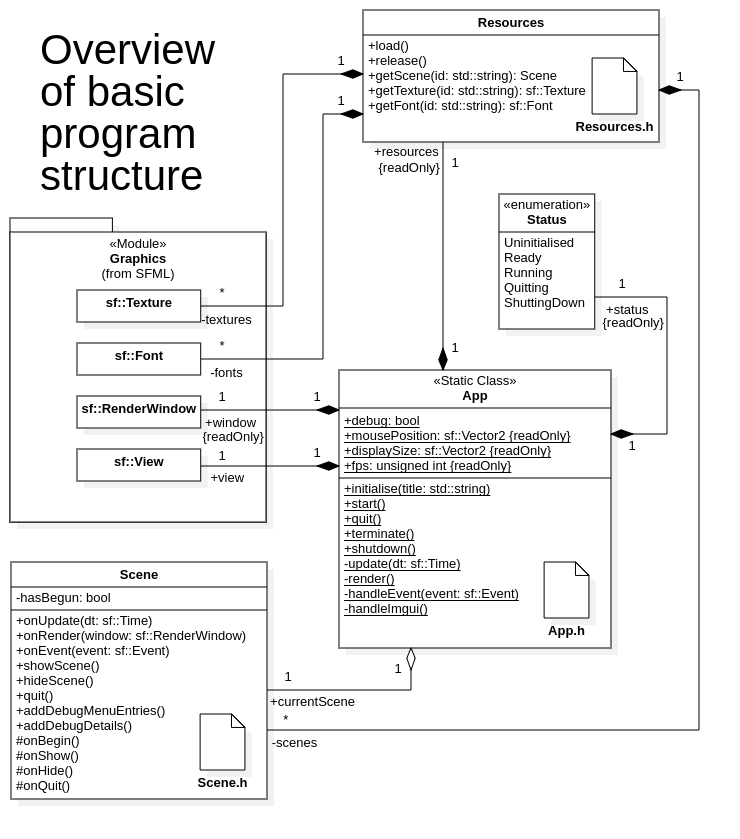
\includegraphics[width=\linewidth]{img/app_overview.png}
  \caption{A UML diagram detailing the infrastructure of the testing environment}
  \label{fig:foundationsUML}
\end{figure}

The first requirement listed in section \ref{subsubsec:requirements} is to create an interactive window that supports 2D graphics. Figure \ref{fig:foundationsUML} illustrates an overview of the program; the \emph{App} class manages the window and handles the main loop of processing input and rendering the screen. The \emph{Scene} class can be inherited to introduce different functionality to the testing environment and will be used to encompass the strategy game and its logic.

\subsubsection{Designing the strategy game}
The second requirement in section \ref{subsubsec:requirements} is to build a sample video game for the AI to play. 

\begin{figure}[!h]
  \centering
  \caption{A UML diagram showing the implementation of the strategy game}
  \label{fig:strategyGameUML}
\end{figure}

END

- Set out requirements and make it clear how these are derived from previous chapters

- Detail design with diagrams, program flow, UML, class headers, interface mock-ups
  - Mention how each requirement is implemented

\subsection {Development (14--15 pages when combined with design)}
\label{subsec:development}

- Go through commit history and summarise main narrative (key milestones and changes). Can always place the rest as a (referenced) appendix.

\subsection {Results and Evaluation (11--12 pages including critical review)}
\label{subsec:resultsAndEvaluation}

- This area can be further subdivided

- Give summary of results in this case, results will be how the AI behaves in each case
  - Evaluate through comparison between other products and other case studies
  - Explain findings, especially if unexpected
 - Discuss further work if applicable
- Demonstrate achievements and indicate how the results meets project requirements
  - Evaluate against criteria with support of gathered data
  - Assess meaning of results of testing 
    - If a criteria has been failed, assess why it did not happen 
      - Was the criteria faulty? If so, explain how knowledge of the problem domain has changed
    - How does what I did prove the criteria?

\section {Conclusions}
\label{sec:conclusions}

\subsection {Conclusions and Critical Review}
\label{subsec:conclusionsAndCriticalReview}

- Compulsory chapter
- (2--3 pages)

- Evaluate to what extent the project objectives have been fulfilled 
- Reflect on the project as a whole 
- Describe limitations 
  - Propose a set of recommendations for improving the methods used
  - Give suggestions for further work
- 'Step away' from the project and assess learning experience
  - If I had to do it again and I knew at the beginning what I know now, what would be different?

\subsection{Conclusions and recommendations}
\label{subsec:conclusionsAndRecommendations}

- This section should briefly summarise:
  - The project objectives
  - Findings
  - Methods used 
  - Deliverable developed
  - Evaluation of the quality of the product
  - Usefulness of the findings
  - Worth of learning experience

\printbibliography[
  heading=bibintoc,
  title={Bibliography}
]
\end{document}
